\documentclass[../../Report.tex]{subfiles}
\usepackage[italian]{babel}


\begin{document}
\chapter{Implementazione}
\label{chap:Implementazione}
In questa parte del report verranno descritte le tecnologie utilizzate per la realizzazione del sistema e le scelte fatte per la sua implementazione.\\

\section{App Mobile}
    Per offrire un'app mobile che possa essere utilizzata sia su sistema operativo Android che iOS abbiamo deciso di utilizzare il framework \emph{Flutter}, un framework open-source sviluppato da Google che si poggia su \emph{Dart}. Il progetto è stato però testato solo su android poichè nessun componente del gruppo possedeva un dispositivo con MacOS. Per la gestione della mappa abbiamo utilizzato il pacchetto \emph{flutter\_map} che permette di integrare comodamente delle mappe Leaflet all'interno delle propria app, mentre per quanto riguarda la libreria per fare Activity Recognition abbiamo utilizzato un pacchetto chiamato \emph{flutter\_Activity\_Recognition}, un wrapper alle librerie di sistema Android e iOs per fare riconoscimento dell'attività dell'utente. \\

\section{Splash Screen}
Lo splash screen è la prima schermata che viene mostrata all'utente quando avvia l'app. Questa schermata è molto semplice e mostra solo il logo dell'app, una semplice icona di un'auto con il nome dell'applicazione. Questa schermata ha lo scopo di intrattenere l'utente durante il caricamento dell'app e di chiedergli i permessi per la localizzazione e per il riconoscimento dell'attività.\\
Mostriamo il codice per la richiesta dei permessi:
\begin{figure}[H]
  \centering
  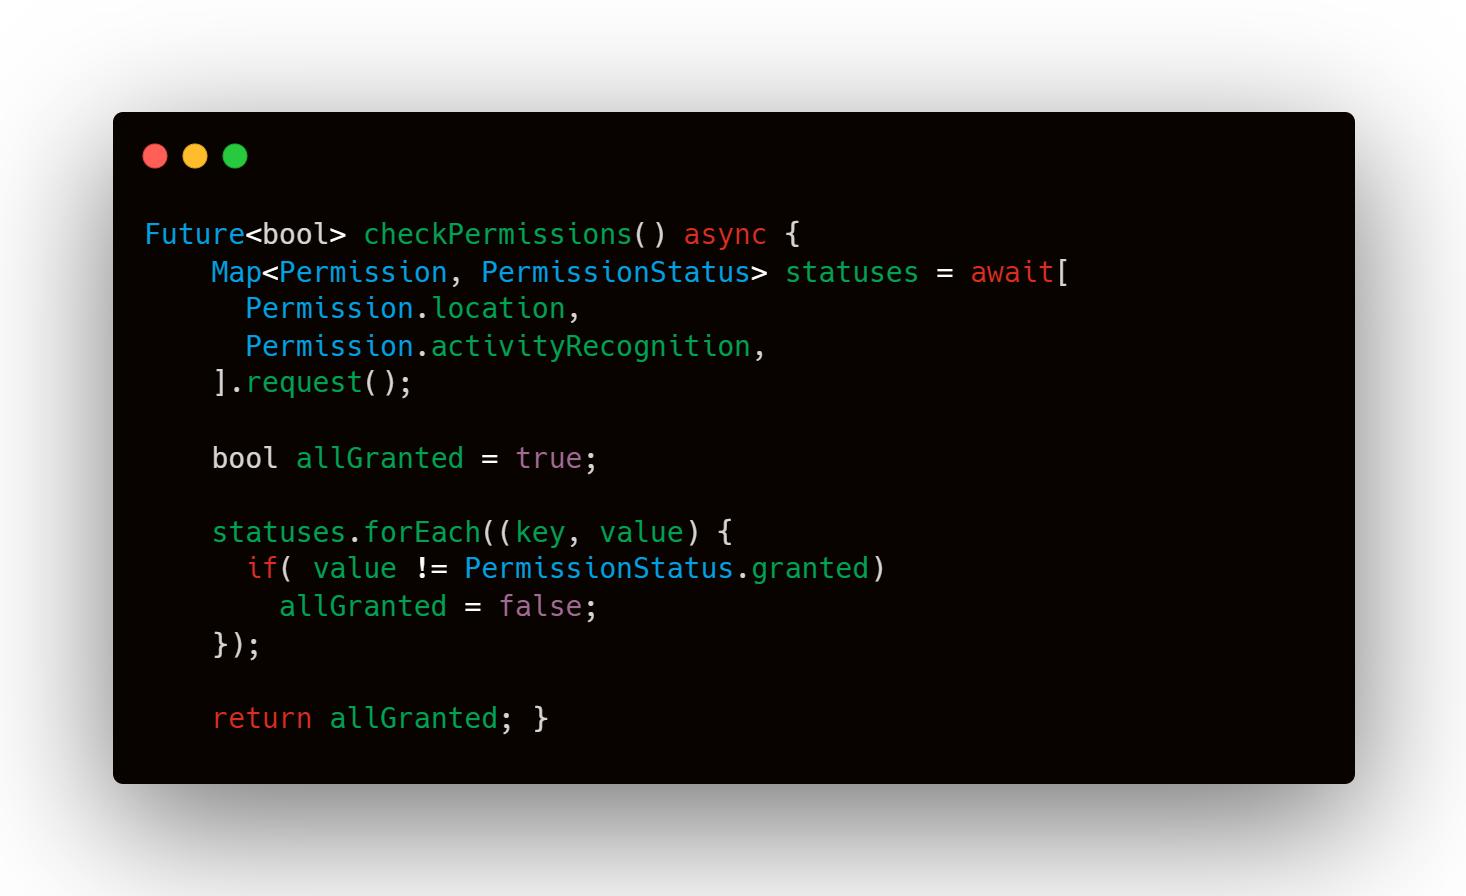
\includegraphics[width=\textwidth]{CheckPermission.png}
  \caption{Codice per la richiesta dei permessi}
\end{figure}
Qualora l'utente non conceda i permessi, invece che caricare Map Widget verrà caricato un altro Widget con un messaggio di errore. \\

\subsection{Activity Recognition}
Per la parte di Activity Recognition, come precedentemente accenato abbiamo utilizzato il pacchetto \emph{flutter\_Activity\_Recognition} che permette di fare riconoscimento dell'attività dell'utente. Il pacchetto riconosce varie attività come: \emph{WALKING}, \emph{RUNNING}, \emph{IN\_BICYCLE}, \emph{IN\_VEICHLE}, \emph{STILL}, \emph{UNKNOWN}. L'implementazione del sistema di activity recognition è stata fatta tramite la classe \emph{ActivityRecognitionClass}. Questa classe viene inizializzata all'interno del MapWidget (la schermata principale dell'app). Al momento della sua inizializzazione questa classe farà partire un listener che farà partire una callback ogni qualvolta viene riconosciuta una nuova attività. Importante notare come verranno eseguite operazioni (aggiornamento dell'attività corrente ed eventuali transizioni) solo dal momento in cui l'attività riconosciuta viene riconosciuta con un grado di confidenza alto. In più, tutto funziona se e solo se l'utente ha dato i permessi all'app di far riconoscere la propria attività.\\
Mostriamo ora il costruttore della classe e la callback che viene eseguita ogni qualvolta viene riconosciuta una nuova attività.\\
\begin{figure}[H]
  \centering
  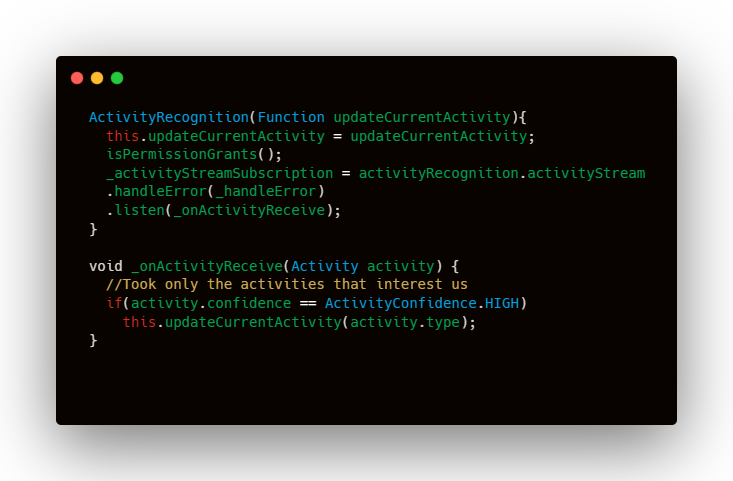
\includegraphics[width=0.8\textwidth]{ActivityRecognitionCode.png}
  \caption{Costruttore e callback di ActivityRecognitionClass}
  \end{figure}

\section{MapWidget}
MapWidget rappresenta la schermata principale dell'applicazione. In questa schermata l'utente può vedere la sua posizione sulla mappa che mostrerà i poligoni. Cliccando su un poligono verrà visualizzato un Toast che indica il numero di parcheggi disponibili per quella zona. Sono inoltre presenti (solo in questa versione Beta dell'app a scopo dimostrativo) dei pulsanti che permettono di simulare l'arrivo e la partenza dall'area di parcheggio, pulsanti che non sarebbero presenti in un'ipotetica versione commerciale dell'app. \\ 
Per la gestione della mappa abbiamo utilizzato il pacchetto \emph{flutter\_map} che permette di integrare comodamente delle mappe Leaflet all'interno delle propria app. Per la visualizzione dei poligoni ci siamo affidati al Layer Polygon di Leaflet, quindi non sono altro che un layer aggiuntivo sulla mappa.\\ 

Il riconoscimento della posizione è stato fatto tramite il pacchetto Geolocator che permette di ottenere la posizione dell'utente in tempo reale.\\

Lato implementativo, questo widget è il widget più importante di tutta l'applicazione. Difatti nell'initState di questo widget esso si occuperà di inizializzare anche altre classi usate all'interno del progetto, come la classe per fare il riconoscimento dell'attività dell'utente. Lo snippet di codice più importante di questa classe è probabilmente la funzione che viene chiamata nella callback del listener dell'activity Recognition: updateCurrentActivity. Questa funzione si occupa di aggiornare l'attività corrente dell'utente e di inviare un messaggio al server per indicare che l'utente è entrato o uscito dall'area di parcheggio.\\
\begin{figure}[H]
  \centering
  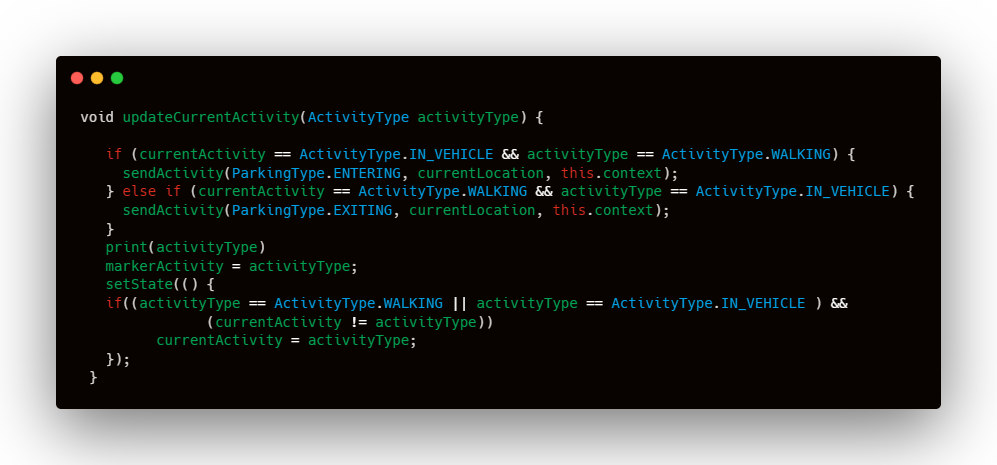
\includegraphics[width=\textwidth]{UpdateCurrentActivity.png}
  \caption{Funzione updateCurrentActivity}
\end{figure}
Lo state currentActivity verrà aggiornato solo se l'attività riconosciuta è \emph{WALKING} o \emph{IN\_VEHICLE} poichè spesso è molto facile che guidando o camminando ci si fermi, portando il sistema a riconoscere l'attività come \emph{STILL}. Questo causerbbe un'impossibilità da parte dell'app di riconoscere un cambiamento netto di attività da \emph{WALKING} a \emph{DRIVING} e viceversa. Tutte le altre attività vengono comunque riconsociute e salvate nella variabile markerActivity che, tramite uno switch permette di cambiare la visualizzazione a schermo, permettendo all'utente di capire quale attività viene riconosciuta in quel momento dal sistema.\\
\begin{figure}[H]
  \centering
  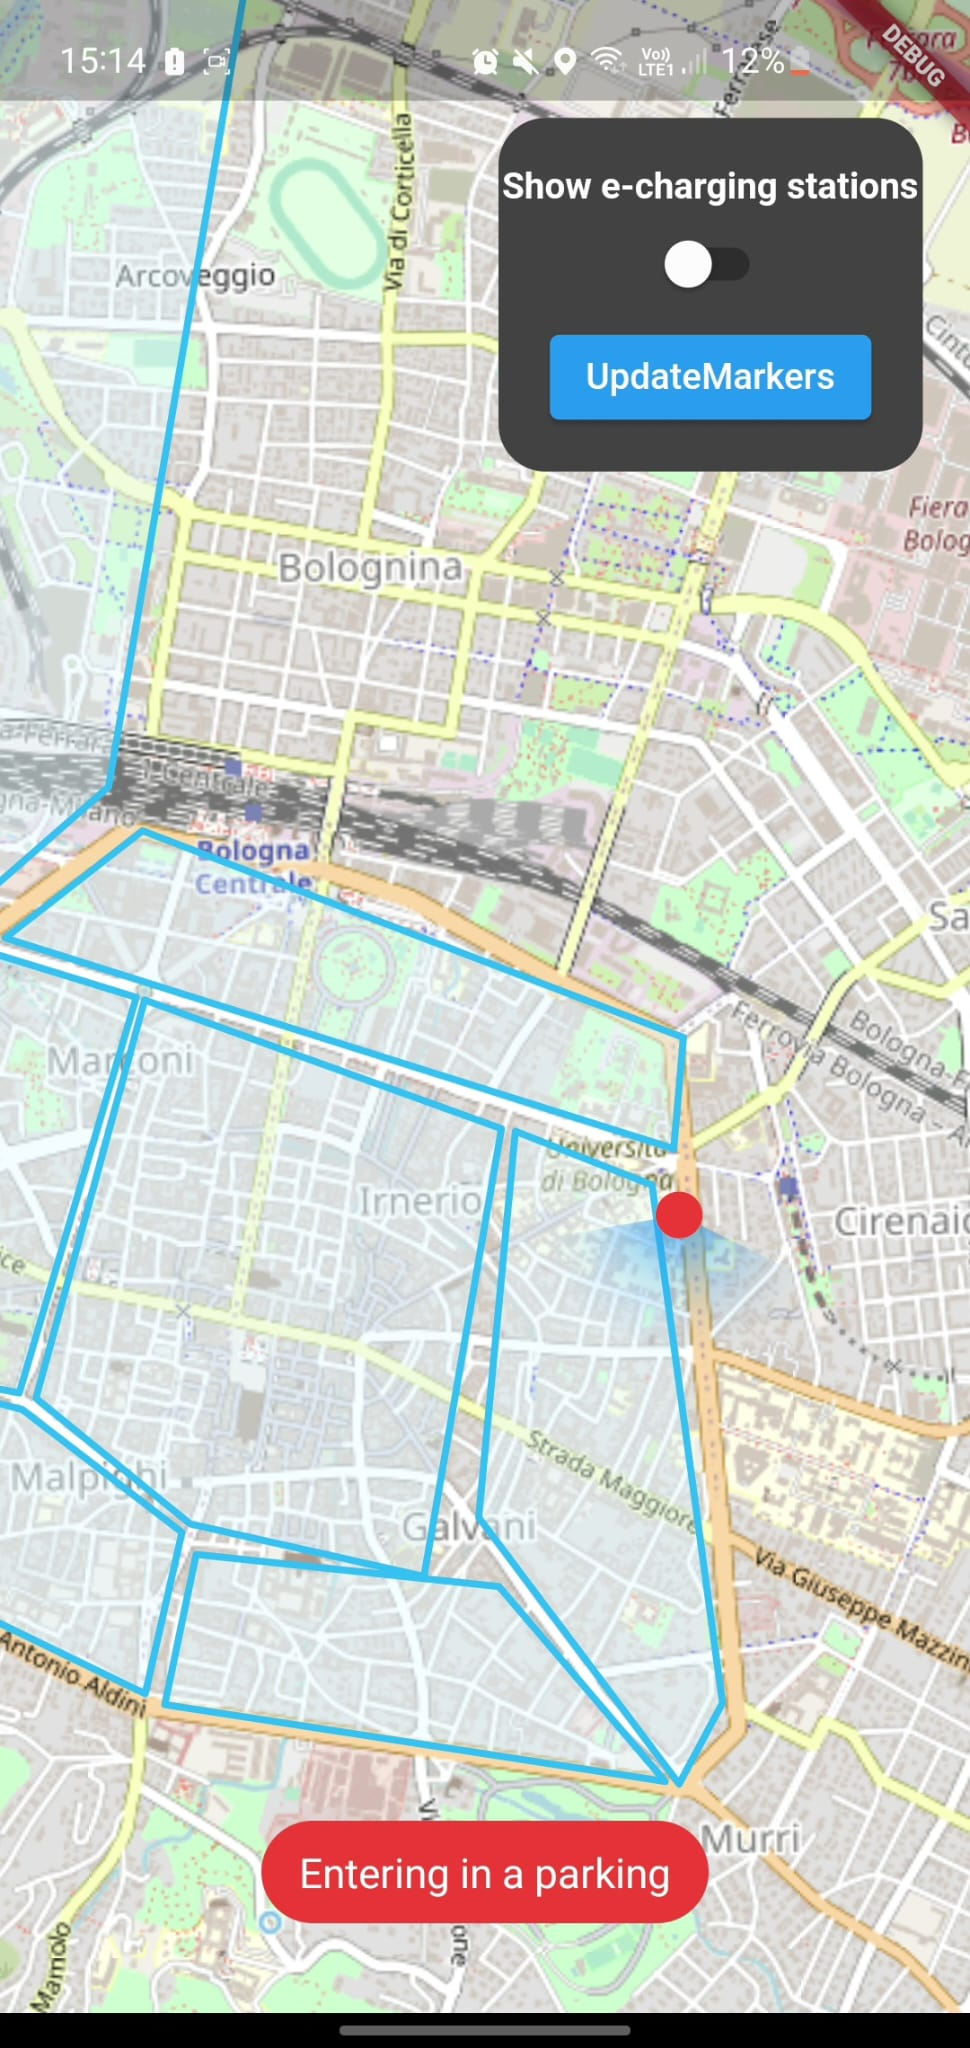
\includegraphics[width=0.3\textwidth]{Entering.jpg}
  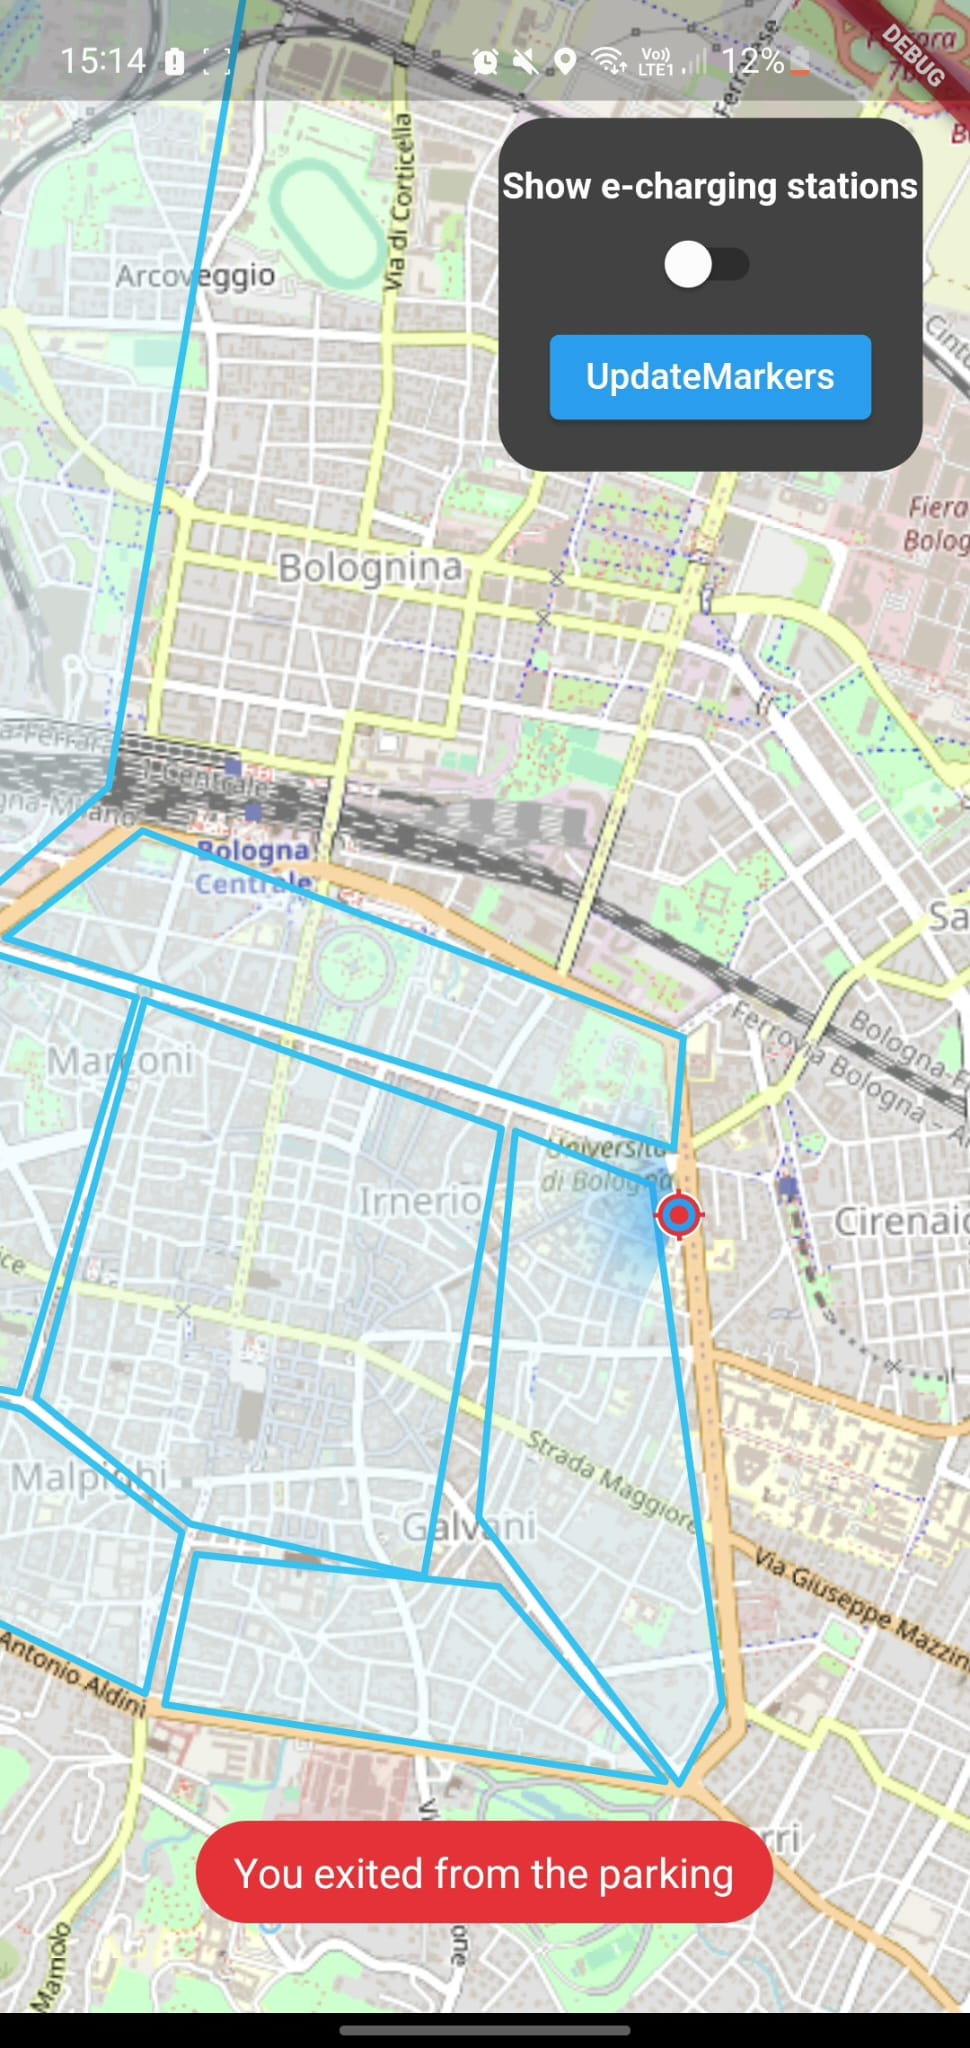
\includegraphics[width=0.3\textwidth]{Exiting.jpg}

  \caption{Riconoscimento di un'entrata e di un'uscita da un parcheggio}
\end{figure}

\subsection{Feature Aggiuntiva}
Lato app mobile, per l'implementazione della feature aggiuntiva ci limitiamo a chiedere al backend i dati relativi alle colonnine elettriche, che visualizzeremo all'interno della mappa.\\ 
Quando un utente parcheggerà il suo veicolo, se si trova in una posizione vicina ad una colonnina elettrica, l'app visualizzerà una dialog che chiederà all'utente se sta utilizzando o meno quella colonnina elettrica. Se l'utente risponde di sì, il backend si occuperà di aggiornare lo stato della colonnina nel database.\\
Mostriamo ora un esempio di questa funzione, tramite una chiamata ad una posizione fissata vicino ad una colonnina elettrica posta in via S.Giacomo: 
\begin{figure}[H]
  \centering
  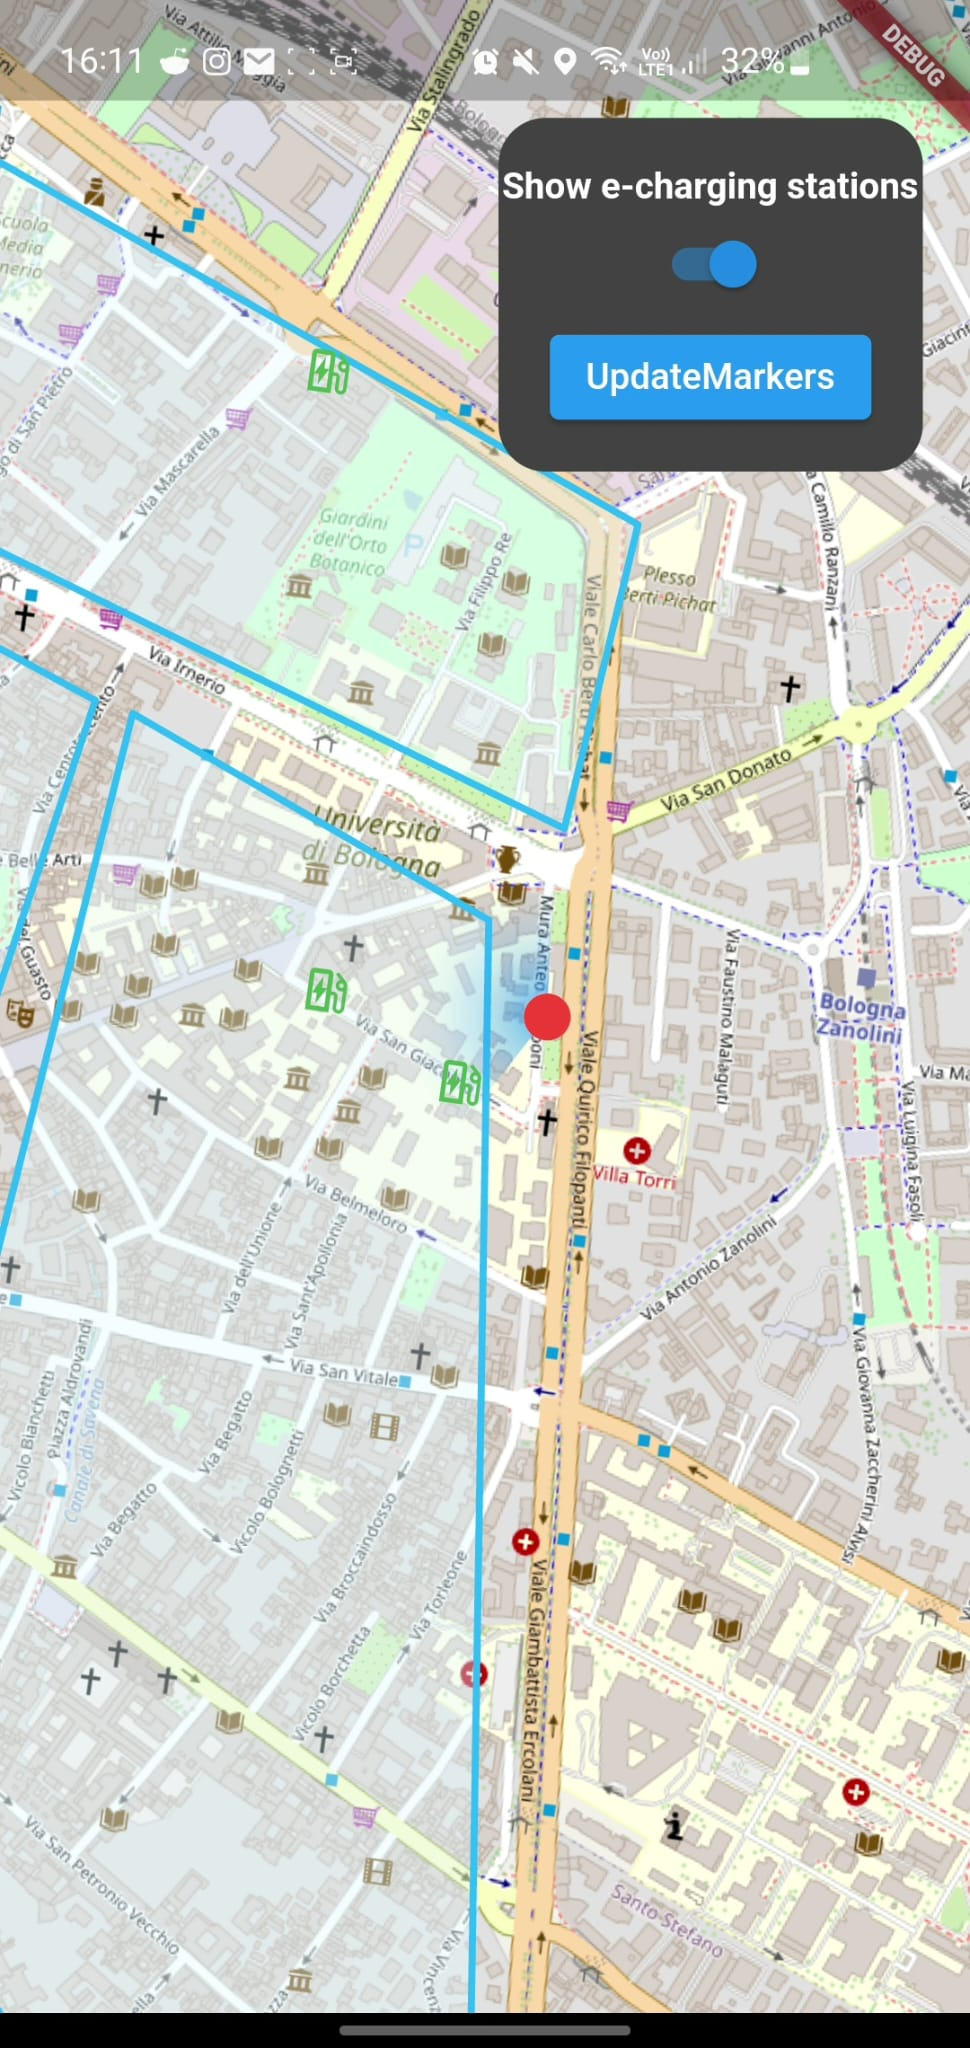
\includegraphics[width=0.3\textwidth]{EnteringE.jpg}
  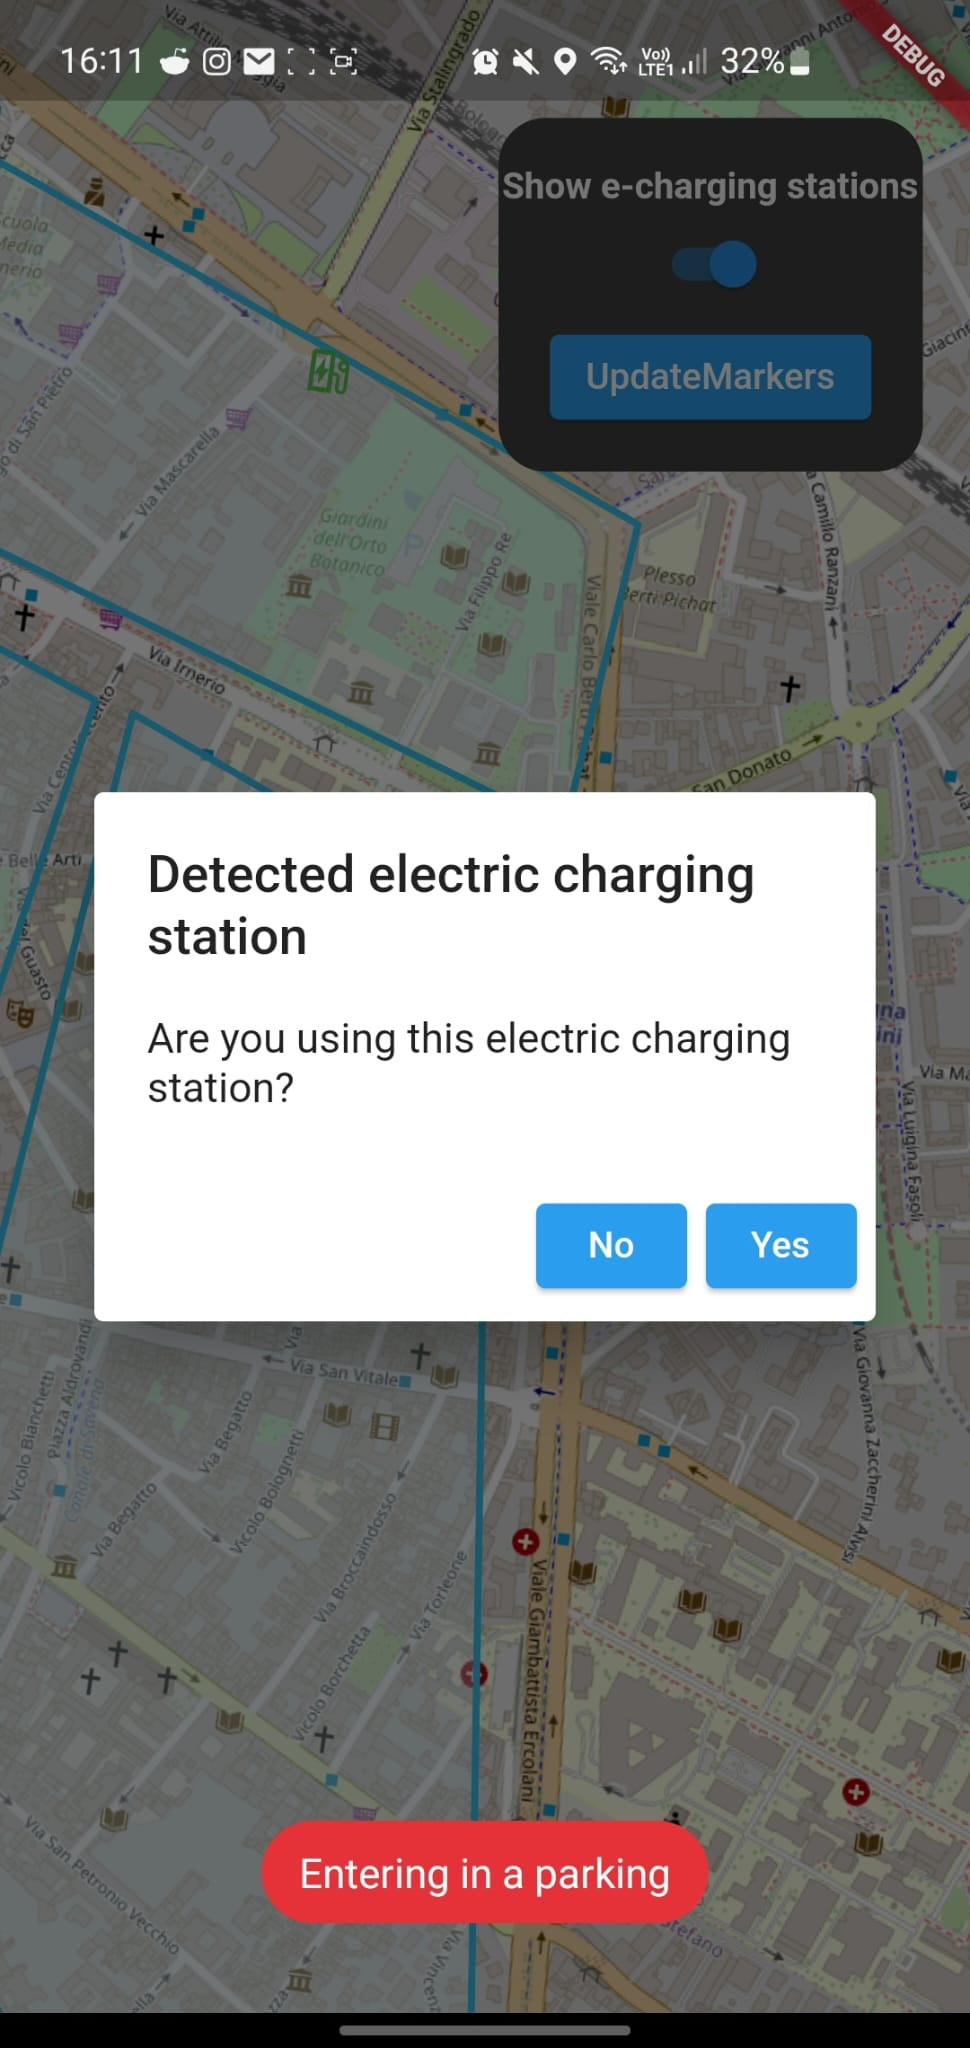
\includegraphics[width=0.3\textwidth]{Dialog.jpg}
  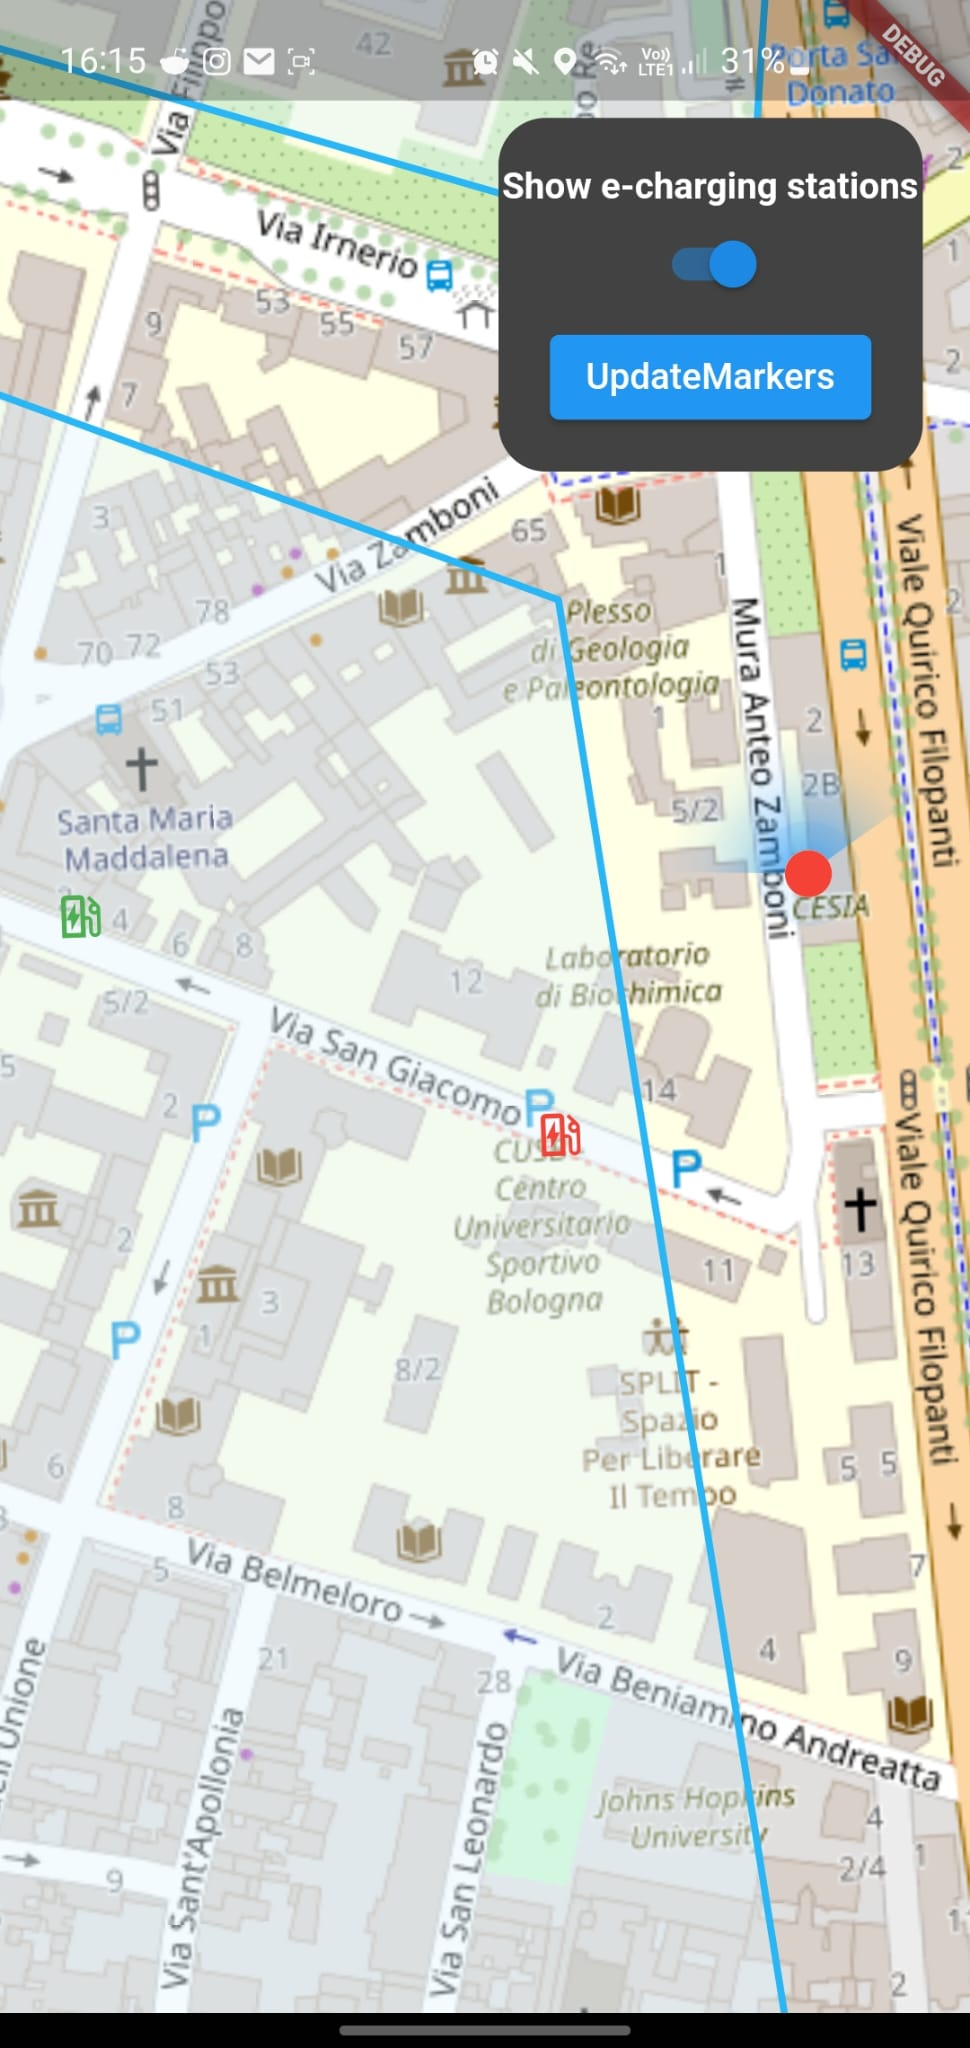
\includegraphics[width=0.3\textwidth]{ExitingE.jpg}

  \caption{Riconoscimento di un'entrata e di un'uscita da un parcheggio nei pressi di una colonnina}
\end{figure}
Dalle immagini si può notare come l'utente sia abbastanza distante dalle colonnine, questo poichè per motivi di test abbiamo deciso di passare una posizione fissata vicina alla colonnina. 



\section{Backend}
    Per il backend abbiamo deciso di utilizzare \emph{Node.js}, un runtime Javascript che permette di creare applicazioni web veloci e scalabili, il Database invece, è stato creato utilizzando \emph{PostgreSQL} con estensione \emph{PostGIS} per la gestione dei dati spaziali.\\
    Lato implementativo abbiamo deciso di dividere il nostro database in moduli, in modo da avere una struttura più pulita e ordinata. Avremo quindi un modulo per la creazione del database, uno per le query e rispettivamente uno per le funzioni esposte al frontend e all'applicazione mobile.\\
    Il nostro database è composto da 5 tabelle e ha questo schema:
    \begin{figure}[H]
      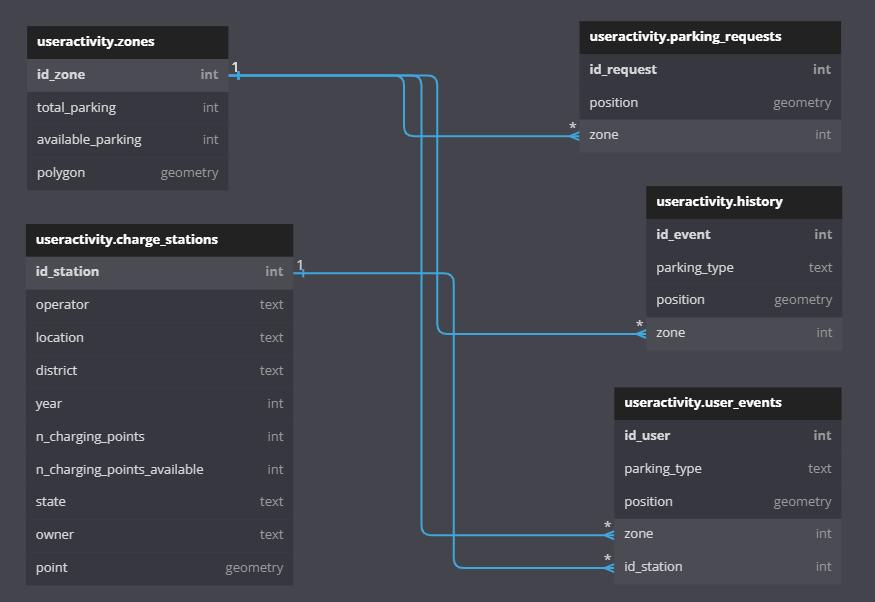
\includegraphics[width=\textwidth]{dbSchema.png}
      \centering
        \caption{Schema del database}
        \label{fig:schema}  
    \end{figure}
    Il database è stato gestito tramite pgAdmin, un software open-source che permette di gestire database PostgreSQL, al quale abbiamo utilizzato anche il plugin PostGIS per la gestione dei dati spaziali.\\
    Entrando nello specifico delle query, mostriamo la query che viene chiamata quando un utente chiede il numero di parcheggi disponibili in una zona:
    \begin{figure}[H]
      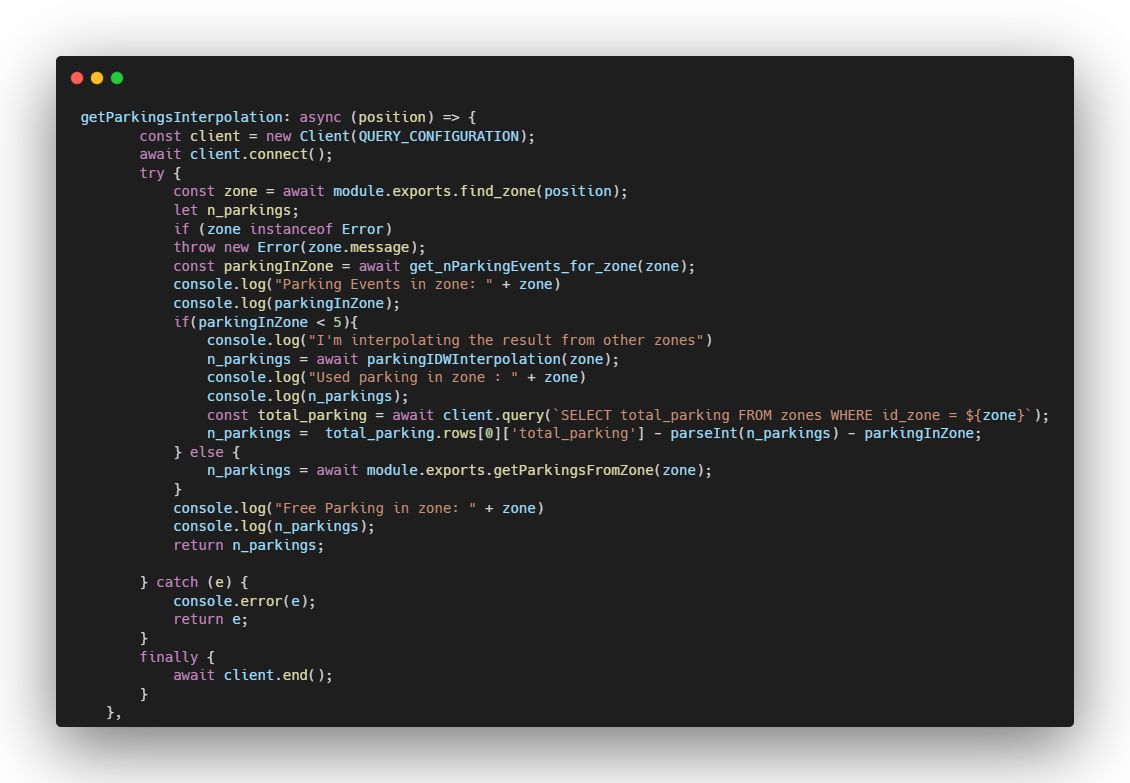
\includegraphics[width=\textwidth]{getParkingsIDW.png}
      \centering
      \caption{Query per il numero di parcheggi disponibili}
      \label{fig:query}
    \end{figure}
    Questa query ci permette di discutere di un'altra importante feature presente nel progetto, l'interpolazione dei parcheggi. Come si può notare dapprima calcoleremo il numero di posti occupati in zona, se questo è minore di 5, un numero molto basso per una città come Bologna dove ci sono molti parcheggi, allora procederemo con l'interpolazione dei dati, altrimenti restituiamo semplicemente il numero di posti liberi in zona.\\
    L'interpolazione dei dati è stata fatta tramite l'algoritmo IDW (Inverse Distance Weighting), un algoritmo che permette di interpolare i dati in base alla distanza tra i punti. Per calcolare la distanza tra due zone, abbiamo dapprima calcolato i centroidi delle zone, poi abbiamo calcolato la distanza tra i centroidi delle zone e infine abbiamo interpolato i dati in base alla distanza tra i centroidi.\\
    Dato un insieme di punti:  
    $ \{\mathbf{x}_i, u_i \mid \text{ per } \mathbf{x}_i \in \mathbb{R}^n, u_i \in \mathbb{R}\}_{i=1}^N $, la funzione di interpolazione $u(\mathbf{x}): \mathbb{R}^n \rightarrow \mathbb{R}$ è definita come:
    $$
    u(\mathbf{x})= 
    \begin{cases}
      \frac{\sum_{i=1}^N w_i(\mathbf{z}) u_i}{\sum_{i=1}^N w_i(\mathbf{x})},
       & \text { if } d(\mathbf{x}, \mathbf{x}_i) \neq 0 \text { per ogni  } i \\
      u_i, & \text{ if } d(\mathbf{x}, \mathbf{x}_i)=0 \text{ per alcune } i
    \end{cases}
    $$
    Dove
    $$
    w_i(\mathbf{x})=\frac{1}{d\left(\mathbf{x}, \mathbf{x}_i\right)}
    $$
    Guardando l'implementazione lato codice:
    \begin{lstlisting}
    SELECT ST_AsText(ST_Centroid(polygon)) FROM zones WHERE id_zone = ${zone}
    \end{lstlisting}
    Questa query ci permette di calcolare il centroide di una zona, dato il suo id.\\
    \begin{figure}[H]
      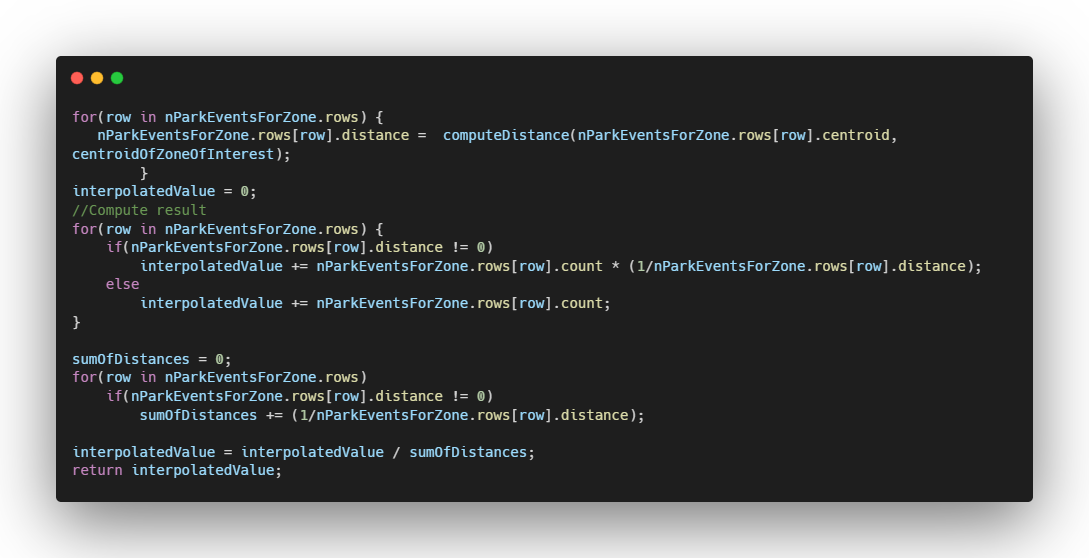
\includegraphics[width=\textwidth]{computeValueIDW.png}
      \centering
      \caption{Calcolo dell'interpolazione dei dati}
      \label{fig:query2}
    \end{figure}
    Questo codice rappresenta invece la computazione effettiva del valore interpolato.\\

\section{Frontend}
    Per  motivi di riusabilità del codice e dei componenti abbiamo deciso di utilizzare il framework React per il frontend, un framework \emph{Javascript} open-source sviluppato da Facebook che permette di creare componenti riutilizzabili. 
    Per la gestione delle mappe nel frontend abbiamo utilizzato la libreria \emph{Leaflet}, un framework Javascript open-source che permette di creare mappe interattive, dal quale abbiamo preso anche due pacchetti per fare Clustering e per visualizzare la Heatmap dei dati. Infine per la parte grafica è stato utilizzato il framework \emph{Material-UI}, un framework Javascript open-source che permette di creare componenti grafici in stile \emph{Material Design}.\\
    Il frontend è composto da tre sezioni, accessibili tramite delle tab in una navbar: 
    \begin{itemize}
      \item La sezione delle richieste: in cui è possibile vedere le zone poligonali di Bologna, selezionarne una e visualizzare il numero di posti liberi in quella zone ed il numero di richieste di parcheggio, cioè quante volte gli utenti hanno chiesto la disponibilità di parcheggi in quella zona.
      \item La sezione della Heatmap: in cui è possibile visualizzare la mappa di Bologna con la heatmap dei dati, cioè il numero di richieste di parcheggio per ogni zona poligonale. La Heatmap è visibile sia complessiva che suddivisa per poligono.
      \item La sezione del Clustering: in cui è possibile visualizzare una visualizzazione dei dati in forma di cluster, cioè dei ragguagliamenti dei dati in base alla loro vicinanza. Sono presenti due visualizzazioni possibili, il clustering K-means e il clusterings DBSCAN. 
    \end{itemize}
    Di seguito mostriamo delle schermate della sezione della Heatmap, sia complessiva che suddivisa per poligono:
    %Two images side by side
    \begin{figure}[H]
        \centering
        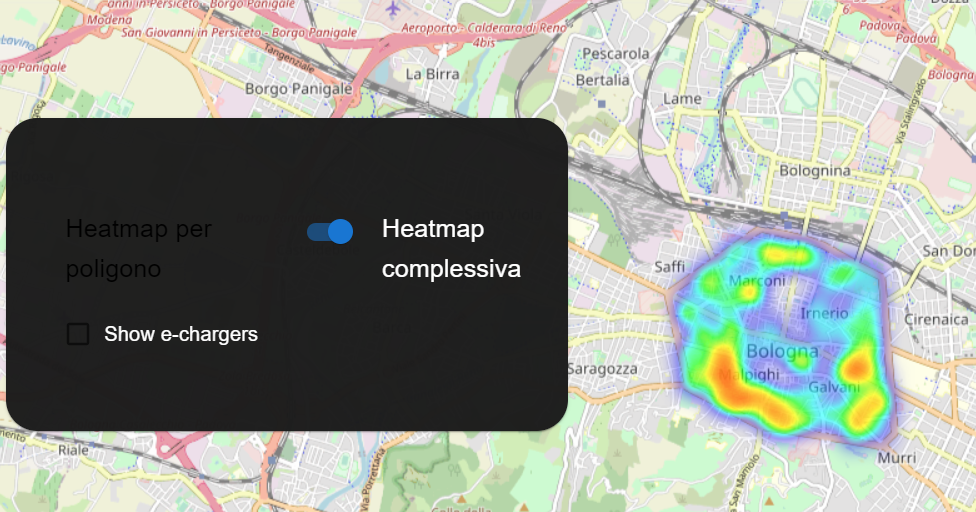
\includegraphics[width=0.52\textwidth]{heatmapFull.png}
        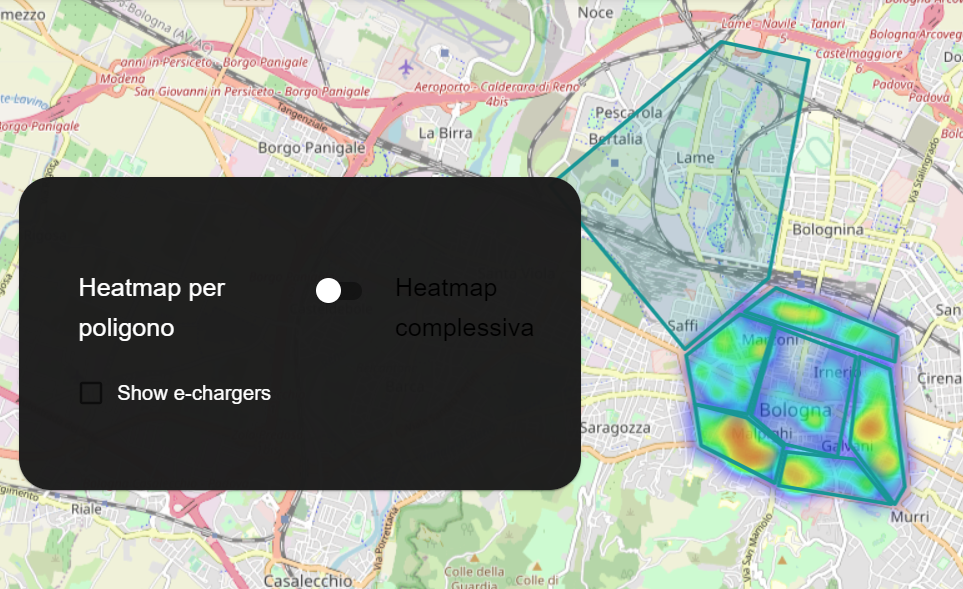
\includegraphics[width=0.45\textwidth]{heatmapPolygons.png}
        \caption{Heatmap complessiva e suddivisa per poligono}
        \label{fig:heatmap}
    \end{figure}
    Mostriamo ora la schermata della sezione del Clustering, in cui è possibile visualizzare i cluster K-means e DBSCAN:
    \begin{figure}[H]
        \centering
        \includegraphics[width=0.45\textwidth]{clusteringKmeans.png}
        \includegraphics[width=0.52\textwidth]{clusteringDBSCAN.png}
        \caption{Schermata della sezione del Clustering}
        \label{fig:clustering}
    \end{figure}
    

    

\end{document}